% Copyright 2004 by Till Tantau <tantau@users.sourceforge.net>.
%
% In principle, this file can be redistributed and/or modified under
% the terms of the GNU Public License, version 2.
%
% However, this file is supposed to be a template to be modified
% for your own needs. For this reason, if you use this file as a
% template and not specifically distribute it as part of a another
% package/program, I grant the extra permission to freely copy and
% modify this file as you see fit and even to delete this copyright
% notice. 

\documentclass{beamer}

% There are many different themes available for Beamer. A comprehensive
% list with examples is given here:
% http://deic.uab.es/~iblanes/beamer_gallery/index_by_theme.html
% You can uncomment the themes below if you would like to use a different
% one:
%\usetheme{AnnArbor}
%\usetheme{Antibes}
%\usetheme{Bergen}
%\usetheme{Berkeley}
%\usetheme{Berlin}
%\usetheme{Boadilla}
%\usetheme{boxes}
%\usetheme{CambridgeUS}
%\usetheme{Copenhagen}
%\usetheme{Darmstadt}
\usetheme{default}
%\usetheme{Frankfurt}
%\usetheme{Goettingen}
%\usetheme{Hannover}
%\usetheme{Ilmenau}
%\usetheme{JuanLesPins}
%\usetheme{Luebeck}
%\usetheme{Madrid}
%\usetheme{Malmoe}
%\usetheme{Marburg}
%\usetheme{Montpellier}
%\usetheme{PaloAlto}
%\usetheme{Pittsburgh}
%\usetheme{Rochester}
%\usetheme{Singapore}
%\usetheme{Szeged}
%\usetheme{Warsaw}

\title{Optimization}

% A subtitle is optional and this may be deleted
\subtitle{Prob:3.14,3.15}

\author{N Chakradhar\inst{1} \and Havish\inst{2}}
% - Give the names in the same order as the appear in the paper.
% - Use the \inst{?} command only if the authors have different
%   affiliation.

\institute[Universities of Somewhere and Elsewhere] % (optional, but mostly needed)
{
  \inst{1}%
  EE16BTECH11022
  \and
  \inst{2}%
  EE16BTECH11023}
% - Use the \inst command only if there are several affiliations.
% - Keep it simple, no one is interested in your street address.


% - Either use conference name or its abbreviation.
% - Not really informative to the audience, more for people (including
%   yourself) who are reading the slides online


% This is only inserted into the PDF information catalog. Can be left
% out. 

% If you have a file called "university-logo-filename.xxx", where xxx
% is a graphic format that can be processed by latex or pdflatex,
% resp., then you can add a logo as follows:

% \pgfdeclareimage[height=0.5cm]{university-logo}{university-logo-filename}
% \logo{\pgfuseimage{university-logo}}

% Delete this, if you do not want the table of contents to pop up at
% the beginning of each subsection:


% Let's get started
\begin{document}

\begin{frame}
  \titlepage
\end{frame}



% Section and subsections will appear in the presentation overview
% and table of contents.

\begin{frame}{Problem 3.14}
  \begin{itemize}
  \item {
Solve
 \begin{align}
\min_x{f(x)} = 4x_1^2 + 2x_2^2
 \end{align}
 with constraints
 \begin{align}
 g_1(x) = 3x_1 + x_2-8 = 0\\
 g_2(x) = 15 - 2x_1 - 4x_2 \leq 0
 \end{align}
  }
  \end{itemize}
\end{frame}

\begin{frame}{Solution}
  Considering the Lagrangian
\begin{align}
L(x,\lambda,\mu) &= f(x) + \lambda g_1(x) + \mu g_2(x) \\
 &= 4x_1^2 + 2x_2^2 + \lambda (3x_1 + x_2-8) + \mu(15 - 2x_1 - 4x_2)\\
 \nabla L(x,\lambda, \mu)  & = 
\begin{pmatrix}
8x_1 + 3 \lambda  -2 \mu  \\
4x_2 + \lambda - 4 \mu \\
3x_1 + x_2 -8 \\
 - 2x_1 - 4x_2 + 15
\end{pmatrix}
= 0
\end{align}
\end{frame}

\begin{frame}{Solution}
resulting in the matrix equation
%
\begin{align}
\Rightarrow 
\begin{pmatrix}
8 &0 & 3 & -2\\
0 &4 & 1 & -4 \\
3 & 1 & 0 &0  \\
2 & 4 & 0 & 0
\end{pmatrix}
\begin{pmatrix}
x_1 \\
x_2 \\
\lambda
\\
\mu
\end{pmatrix}
&=
\begin{pmatrix}
0 \\
0 \\
8 \\
15
\end{pmatrix}
\\
\Rightarrow 
\begin{pmatrix}
x_1 \\
x_2 \\
\lambda
\\
\mu
\end{pmatrix}
&= 
\begin{pmatrix}
1.7 \\
 2.9 \\
-3.12 \\
2.12
\end{pmatrix}
\end{align}
\end{frame}

\begin{frame}{Observations}
\begin{itemize}
\item The solution $(x_1,x_2)$ is a feasible local minima.
\item The value of $\mu$ is positive.
\item The feasible solution lies on the boundary of the inequality
\end{itemize}
\begin{figure}[!ht]
\centering
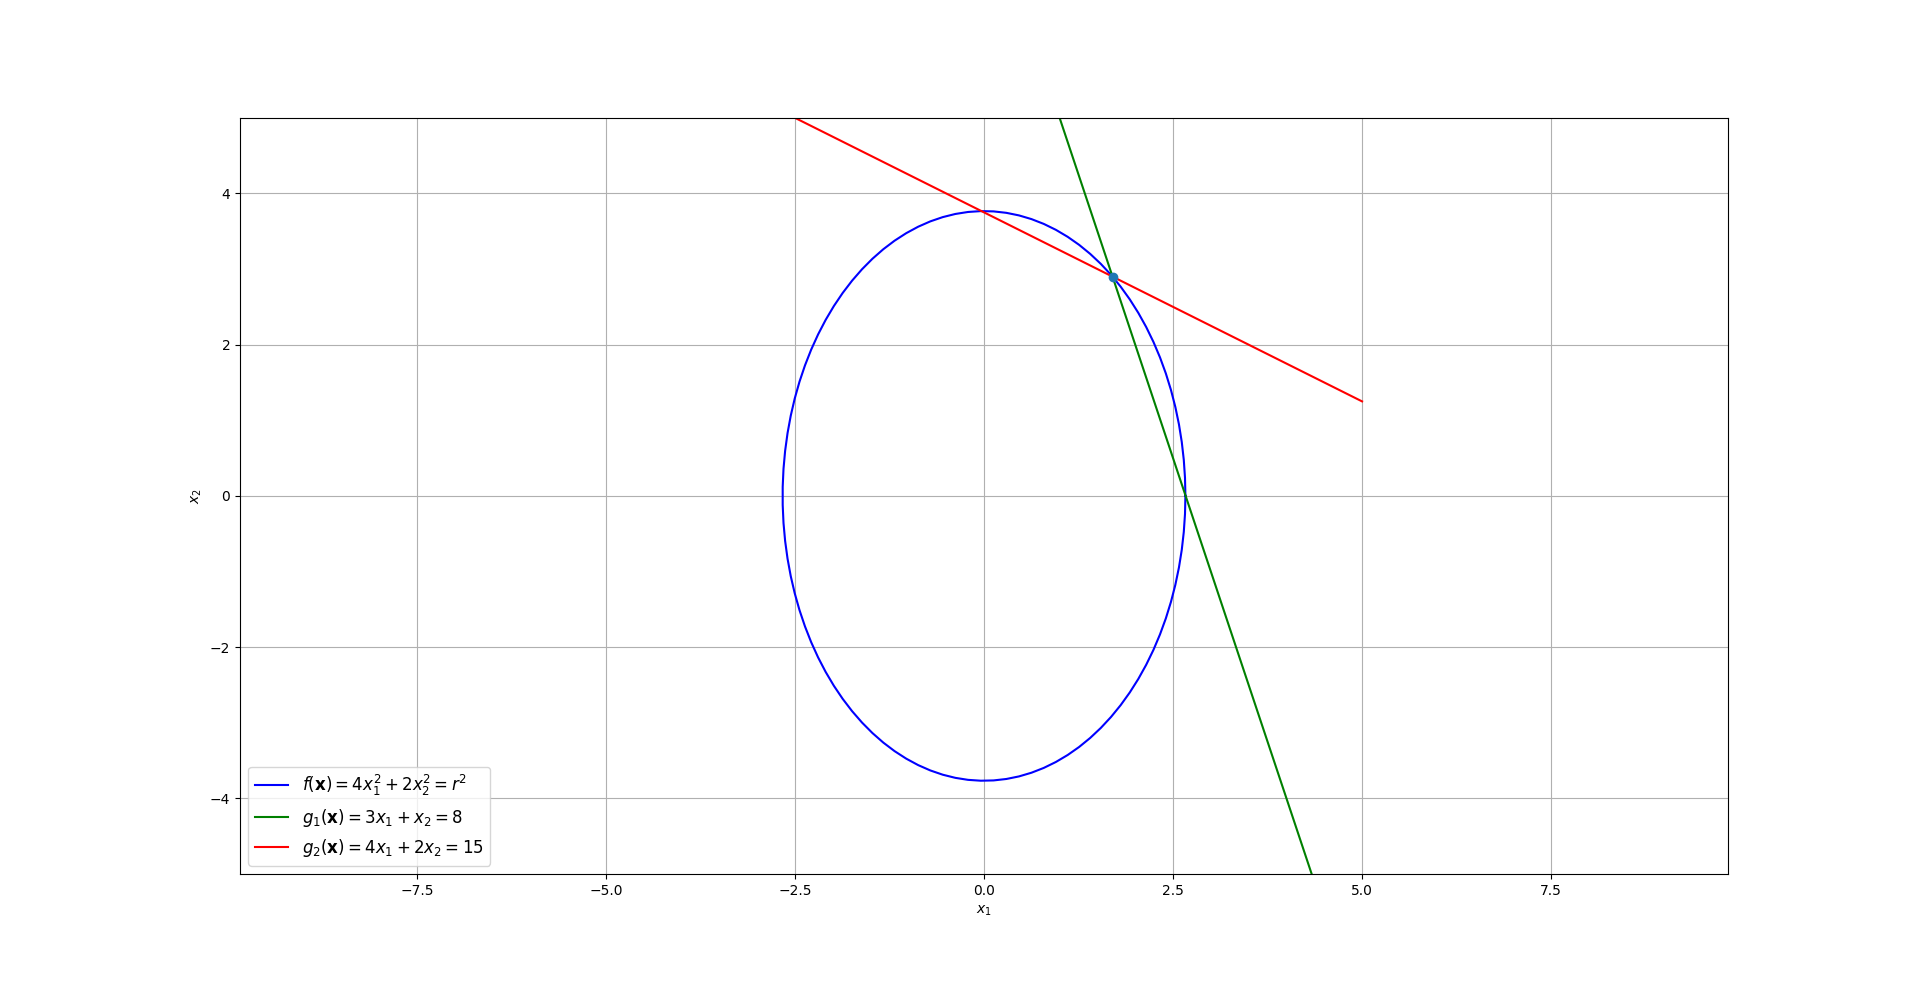
\includegraphics[width=\columnwidth]{./1.png}
\caption{ Correct solution is at intersection of the two lines $r = 5.33$}
\end{figure}
\end{frame}



\begin{frame}{Problem 3.15}
Steps to solve convex optimization problems using Lagrange Multipliers  
    \begin{align}
	x^* &= \min_xf(x)
	\\
	\text{subject to } h_i(x) &= 0, \forall i=1,..,m
	\\
	\text{subject to } g_i(x) &\le 0, \forall i=1,..,n
	\end{align}
	the optimal solution is obtained by considering the following
	\begin{align}
	x^* &= \min_xL(x,\vec{\lambda},\vec{\mu)} 
\\
&= \min_xf(x)  + \underset{i=1}{\overset{m}{\sum}} \lambda_i h_i(x) + \underset{i=1}{\overset{n}{\sum}} \mu_i g_i(x)
\end{align}

\end{frame}

\begin{frame}{Problem 3.15}
\begin{align}
\Rightarrow \nabla f(x) +\underset{i=1}{\overset{m}{\sum}}\lambda_i \nabla  h_i(x) + \underset{i=1}{\overset{n}{\sum}} \mu_i \nabla   g_i(x) = 0
\\
\end{align}
The solution to the above equation should satisfy the below conditions to be feasible:
\begin{align}
 \mu_i g_i(x) &= 0, \forall i=1,..,m
	\\
\text{and } \mu_i &\ge 0, \forall i=1,..,m
\end{align}
It can be verified that the solution obtained in problem 3.14 satisfies the above conditions and hence it is a feasible solution.
\end{frame}
\end{document}


